\documentclass[color=usenames,dvipsnames]{beamer}\usepackage[]{graphicx}\usepackage[]{color}
% maxwidth is the original width if it is less than linewidth
% otherwise use linewidth (to make sure the graphics do not exceed the margin)
\makeatletter
\def\maxwidth{ %
  \ifdim\Gin@nat@width>\linewidth
    \linewidth
  \else
    \Gin@nat@width
  \fi
}
\makeatother

\definecolor{fgcolor}{rgb}{0, 0, 0}
\newcommand{\hlnum}[1]{\textcolor[rgb]{0.69,0.494,0}{#1}}%
\newcommand{\hlstr}[1]{\textcolor[rgb]{0.749,0.012,0.012}{#1}}%
\newcommand{\hlcom}[1]{\textcolor[rgb]{0.514,0.506,0.514}{\textit{#1}}}%
\newcommand{\hlopt}[1]{\textcolor[rgb]{0,0,0}{#1}}%
\newcommand{\hlstd}[1]{\textcolor[rgb]{0,0,0}{#1}}%
\newcommand{\hlkwa}[1]{\textcolor[rgb]{0,0,0}{\textbf{#1}}}%
\newcommand{\hlkwb}[1]{\textcolor[rgb]{0,0.341,0.682}{#1}}%
\newcommand{\hlkwc}[1]{\textcolor[rgb]{0,0,0}{\textbf{#1}}}%
\newcommand{\hlkwd}[1]{\textcolor[rgb]{0.004,0.004,0.506}{#1}}%
\let\hlipl\hlkwb

\usepackage{framed}
\makeatletter
\newenvironment{kframe}{%
 \def\at@end@of@kframe{}%
 \ifinner\ifhmode%
  \def\at@end@of@kframe{\end{minipage}}%
  \begin{minipage}{\columnwidth}%
 \fi\fi%
 \def\FrameCommand##1{\hskip\@totalleftmargin \hskip-\fboxsep
 \colorbox{shadecolor}{##1}\hskip-\fboxsep
     % There is no \\@totalrightmargin, so:
     \hskip-\linewidth \hskip-\@totalleftmargin \hskip\columnwidth}%
 \MakeFramed {\advance\hsize-\width
   \@totalleftmargin\z@ \linewidth\hsize
   \@setminipage}}%
 {\par\unskip\endMakeFramed%
 \at@end@of@kframe}
\makeatother

\definecolor{shadecolor}{rgb}{.97, .97, .97}
\definecolor{messagecolor}{rgb}{0, 0, 0}
\definecolor{warningcolor}{rgb}{1, 0, 1}
\definecolor{errorcolor}{rgb}{1, 0, 0}
\newenvironment{knitrout}{}{} % an empty environment to be redefined in TeX

\usepackage{alltt}
%\documentclass[color=usenames,dvipsnames,handout]{beamer}

\usepackage[roman]{../lectures}
%\usepackage[sans]{../lectures}


\hypersetup{pdfpagemode=UseNone,pdfstartview={FitV}}


% Load function to compile and open PDF


% Compile and open PDF






%% New command for inline code that isn't to be evaluated
\definecolor{inlinecolor}{rgb}{0.878, 0.918, 0.933}
\newcommand{\inr}[1]{\colorbox{inlinecolor}{\texttt{#1}}}
\IfFileExists{upquote.sty}{\usepackage{upquote}}{}
\begin{document}



\begin{frame}[plain]
  \LARGE
%  \maketitle
  \centering
  {\huge %Lecture 13 \\
    Dynamic occupancy models} \\
  {\color{default} \rule{\textwidth}{0.1pt}}
  \vfill
  \large
  WILD(FISH) 8390 \\
  Estimation of Fish and Wildlife Population Parameters \\
  \vfill
  Richard Chandler \\
  University of Georgia \\
\end{frame}






\section{Overview}



\begin{frame}[plain]
  \frametitle{Outline}
  \Large
  \only<1>{\tableofcontents}%[hideallsubsections]}
  \only<2 | handout:0>{\tableofcontents[currentsection]}%,hideallsubsections]}
\end{frame}



\begin{frame}
  \frametitle{Overview}
  When we covered static occupancy models, we focused exclusively on
  spatial variation. \\   
  \pause
  \vfill
  Historically, the study of population dynamics was entirely
  focused on temporal variation. \\
  \pause
  \vfill
  Metapopulation models played a big role in emphasizing both spatial
  and temporal dynamics. \\
  \pause
  \vfill
  Dynamic occupancy models allow for inference on spatio-temporal
  occupancy resulting from local colonization and extinction
  processes. \\
\end{frame}





\begin{frame}
  \frametitle{Static (single-season) occupancy model}
  {\centering \color{blue} Refresher \\}
  \vfill
  \small
  The model for the state process is the same as logistic regression:
  \begin{gather*}
    \mathrm{logit}(\psi_i) = \beta_0 + \beta_1 x_{i1} + \beta_2 x_{i2} + \cdots \\
    z_i \sim \mathrm{Bern}(\psi_i)
  \end{gather*}
  \pause
  \vfill
  Model for the observation process conditional on the state process:
  \begin{gather*}
    \mathrm{logit}(p_{ij}) = \alpha_0 + \alpha_1 x_{ij1} + \alpha_2 x_{ij2} + \cdots \\
    y_{ij} \sim \mathrm{Bern}(z_i\times p_{ij})
  \end{gather*}
  \pause
  Definitions \\
  $\psi_i$ -- probability that the species occurs at site $i$ \\
  $z_i$ -- binary presence/absence variable at site $i$ \\
  $p_{ij}$ -- probability of detecting the species at site $i$ on occasion $j$ \\
  $y_{ij}$ -- binary detection/non-detection data
\end{frame}



\begin{frame}
  \frametitle{Dynamic occupancy model}
  \small
  Initial occupancy state (same as static model), for $k=1$.
  \begin{gather*}
    z_{i,1} \sim \mathrm{Bern}(\psi_{i,1})
  \end{gather*}
  \pause
%  \vfill
  Occupancy state dynamics, for $k=2, \dots, K$.
  \begin{gather*}
    \psi_{i,k} = z_{i,k-1}(1-\varepsilon) +  (1-z_{i,k-1})\gamma \\
    z_{i,k} \sim \mathrm{Bern}(\psi_{i,k})
  \end{gather*}
  \pause
%  \vfill
  Observation model
  \begin{gather*}
    y_{i,j,k} \sim \mathrm{Bern}(z_{i,k}\times p)
  \end{gather*}
  \pause
%  Definitions \\
  \footnotesize
  $\psi_{i,k}$ -- probability species occurs at site $i$ during primary period $k$ \\
  $z_{i,k}$ -- binary presence/absence variable \\
  $\varepsilon$ -- local extinction probability \\
  $\gamma$ -- local colonization probability \\
  $p$ -- probability of detecting the species if it's present \\
  $y_{i,j,k}$ -- detection data at site $i$ on secondary period $j$, primary period $k$ \\
  \pause \vfill
  \centering
  \small
  You can model $\psi_1$, $\varepsilon$, $\gamma$, and $p$ as
  functions of covariates \\
\end{frame}


%\section{Simulation}



\begin{frame}
  \frametitle{Colonization and extinction dynamics}
  \small
  After the initial time period, the probability that a site is
  occupied depends on the previous state and the two probabilities:
  \pause
  \begin{enumerate}
    \item<2-> Local colonization: $\gamma=\Pr(z_{i,k}=1|z_{i,k-1}=0)$
    \item<3-> Local extinction: $\varepsilon=\Pr(z_{i,k}=0|z_{i,k-1}=1)$
  \end{enumerate}
  {\centering
    \uncover<4->{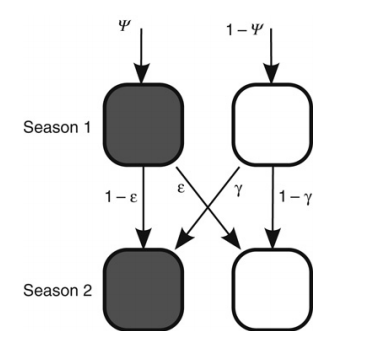
\includegraphics[width=0.3\textwidth]{figure/royle_dorazio_9-1} \\
    \scriptsize From Royle and Dorazio (2008)}  \\
  }
  \vfill
  \uncover<5->{These probabilities can depend on spatio-temporal
    covariates and random effects. In spatially-explicit models, they
    depend on the states and distances to neighboring sites.}
\end{frame}


\section{Without covariates}


\begin{frame}
  \frametitle{Outline}
  \Large
  \tableofcontents[currentsection]
\end{frame}


\begin{frame}[fragile]
  \frametitle{Simulation without covariates}
  \small
%  No covariates
  \vfill
  \begin{enumerate}[<+->]
    \small
  \item Initial occupancy
\begin{knitrout}\scriptsize
\definecolor{shadecolor}{rgb}{0.878, 0.918, 0.933}\color{fgcolor}\begin{kframe}
\begin{alltt}
\hlstd{nSites} \hlkwb{<-} \hlnum{100}
\hlstd{nPrimary} \hlkwb{<-} \hlnum{10}
\hlstd{z} \hlkwb{<-} \hlstd{psi} \hlkwb{<-} \hlkwd{matrix}\hlstd{(}\hlnum{NA}\hlstd{, nSites, nPrimary)}
\hlstd{psi[,}\hlnum{1}\hlstd{]} \hlkwb{<-} \hlnum{0.5}  \hlcom{## Initial occupancy prob}
\hlstd{z[,}\hlnum{1}\hlstd{]} \hlkwb{<-} \hlkwd{rbinom}\hlstd{(}\hlkwc{n}\hlstd{=nSites,} \hlkwc{size}\hlstd{=}\hlnum{1}\hlstd{,} \hlkwc{prob}\hlstd{=psi[,}\hlnum{1}\hlstd{])}
\end{alltt}
\end{kframe}
\end{knitrout}
  \item Occupancy dynamics
\begin{knitrout}\scriptsize
\definecolor{shadecolor}{rgb}{0.878, 0.918, 0.933}\color{fgcolor}\begin{kframe}
\begin{alltt}
\hlstd{epsilon} \hlkwb{<-} \hlnum{0.3} \hlcom{## Local extinction prob}
\hlstd{gamma} \hlkwb{<-} \hlnum{0.2}   \hlcom{## Local colonization prob}
\hlkwa{for}\hlstd{(k} \hlkwa{in} \hlnum{2}\hlopt{:}\hlstd{nPrimary) \{}
    \hlstd{psi[,k]} \hlkwb{<-} \hlstd{z[,k}\hlopt{-}\hlnum{1}\hlstd{]}\hlopt{*}\hlstd{(}\hlnum{1}\hlopt{-}\hlstd{epsilon)} \hlopt{+} \hlstd{(}\hlnum{1}\hlopt{-}\hlstd{z[,k}\hlopt{-}\hlnum{1}\hlstd{])}\hlopt{*}\hlstd{gamma}
    \hlstd{z[,k]} \hlkwb{<-} \hlkwd{rbinom}\hlstd{(}\hlkwc{n}\hlstd{=nSites,} \hlkwc{size}\hlstd{=}\hlnum{1}\hlstd{,} \hlkwc{prob}\hlstd{=psi[,k])    \}}
\end{alltt}
\end{kframe}
\end{knitrout}
  \item Data
\begin{knitrout}\scriptsize
\definecolor{shadecolor}{rgb}{0.878, 0.918, 0.933}\color{fgcolor}\begin{kframe}
\begin{alltt}
\hlstd{nSecondary} \hlkwb{<-} \hlnum{3}
\hlstd{p} \hlkwb{<-} \hlnum{0.2}
\hlstd{y} \hlkwb{<-} \hlkwd{array}\hlstd{(}\hlnum{NA}\hlstd{,} \hlkwd{c}\hlstd{(nSites, nSecondary, nPrimary))}
\hlkwa{for}\hlstd{(i} \hlkwa{in} \hlnum{1}\hlopt{:}\hlstd{nSites) \{}
    \hlkwa{for}\hlstd{(k} \hlkwa{in} \hlnum{1}\hlopt{:}\hlstd{nPrimary) \{}
        \hlstd{y[i,,k]} \hlkwb{<-} \hlkwd{rbinom}\hlstd{(nSecondary,} \hlkwc{size}\hlstd{=}\hlnum{1}\hlstd{,} \hlkwc{prob}\hlstd{=z[i,k]}\hlopt{*}\hlstd{p)}
    \hlstd{\} \}}
\end{alltt}
\end{kframe}
\end{knitrout}
\end{enumerate}
\end{frame}




\begin{frame}[fragile]
  \frametitle{Simulated data}
  \begin{columns}
    \begin{column}{0.4\textwidth}
      \small
      Observations
%      \tiny
\begin{knitrout}\scriptsize
\definecolor{shadecolor}{rgb}{0.878, 0.918, 0.933}\color{fgcolor}\begin{kframe}
\begin{alltt}
\hlstd{y[}\hlnum{1}\hlopt{:}\hlnum{15}\hlstd{,,}\hlnum{1}\hlstd{]}
\end{alltt}
\begin{verbatim}
##       [,1] [,2] [,3]
##  [1,]    0    0    0
##  [2,]    0    0    0
##  [3,]    0    0    0
##  [4,]    1    0    0
##  [5,]    0    1    0
##  [6,]    0    0    0
##  [7,]    0    1    0
##  [8,]    0    0    0
##  [9,]    0    0    0
## [10,]    0    0    0
## [11,]    0    0    1
## [12,]    0    0    0
## [13,]    0    0    0
## [14,]    0    0    0
## [15,]    0    0    0
\end{verbatim}
\end{kframe}
\end{knitrout}
  \end{column}
  \begin{column}{0.6\textwidth}
    \pause
%    \scriptsize
    {\centering Summary stats \\}
    \vspace{24pt}
  Detections at each site \\
\begin{knitrout}\scriptsize
\definecolor{shadecolor}{rgb}{0.878, 0.918, 0.933}\color{fgcolor}\begin{kframe}
\begin{alltt}
\hlstd{siteDets} \hlkwb{<-} \hlkwd{rowSums}\hlstd{(y)} \hlcom{# Dets at each site}
\hlkwd{table}\hlstd{(siteDets)}        \hlcom{# Frequency}
\end{alltt}
\begin{verbatim}
## siteDets
##  0  1  2  3  4  5  6  7  9 
## 17 20 20 17 13  4  5  3  1
\end{verbatim}
\end{kframe}
\end{knitrout}
\pause
\vfill
\small
Detections each year \\
\begin{knitrout}\scriptsize
\definecolor{shadecolor}{rgb}{0.878, 0.918, 0.933}\color{fgcolor}\begin{kframe}
\begin{alltt}
\hlstd{yearDets} \hlkwb{<-} \hlkwd{apply}\hlstd{(y,} \hlnum{3}\hlstd{, sum)}
\hlstd{yearDets}
\end{alltt}
\begin{verbatim}
##  [1] 27 30 31 28 22 15 22 27 20 21
\end{verbatim}
\end{kframe}
\end{knitrout}

  \end{column}
  \end{columns}
\end{frame}



% \begin{frame}
%   \frametitle{Outline}
%   \Large
%   \tableofcontents[currentsection]
% \end{frame}



\subsection{Likelihood}



\begin{frame}[fragile]
  \frametitle{Prepare data in `unmarked'}
  \small
Notice the new argument \inr{numPrimary}:
\begin{knitrout}\scriptsize
\definecolor{shadecolor}{rgb}{0.878, 0.918, 0.933}\color{fgcolor}\begin{kframe}
\begin{alltt}
\hlcom{## Format as nSites by (nSec*nPrimary) matrix}
\hlstd{y.wide} \hlkwb{<-} \hlkwd{matrix}\hlstd{(y,} \hlkwc{nrow}\hlstd{=}\hlkwd{nrow}\hlstd{(y))}
\hlstd{umf} \hlkwb{<-} \hlkwd{unmarkedMultFrame}\hlstd{(}\hlkwc{y}\hlstd{=y.wide,} \hlkwc{numPrimary}\hlstd{=nPrimary)}
\end{alltt}
\end{kframe}
\end{knitrout}
\pause

\begin{knitrout}\scriptsize
\definecolor{shadecolor}{rgb}{0.878, 0.918, 0.933}\color{fgcolor}\begin{kframe}
\begin{alltt}
\hlkwd{summary}\hlstd{(umf)}
\end{alltt}
\begin{verbatim}
## unmarkedFrame Object
## 
## 100 sites
## Maximum number of observations per site: 30 
## Mean number of observations per site: 30 
## Number of primary survey periods: 10 
## Number of secondary survey periods: 3 
## Sites with at least one detection: 83 
## 
## Tabulation of y observations:
##    0    1 
## 2757  243
\end{verbatim}
\end{kframe}
\end{knitrout}
\end{frame}




\begin{frame}[fragile]
  \frametitle{Fit the model}
  \footnotesize
  Notice the 4 distinct formulas
\begin{knitrout}\tiny
\definecolor{shadecolor}{rgb}{0.878, 0.918, 0.933}\color{fgcolor}\begin{kframe}
\begin{alltt}
\hlstd{fm} \hlkwb{<-} \hlkwd{colext}\hlstd{(}\hlopt{~}\hlnum{1}\hlstd{,}\hlopt{~}\hlnum{1}\hlstd{,}\hlopt{~}\hlnum{1}\hlstd{,}\hlopt{~}\hlnum{1}\hlstd{, umf)}
\hlstd{fm}
\end{alltt}
\begin{verbatim}
## 
## Call:
## colext(psiformula = ~1, gammaformula = ~1, epsilonformula = ~1, 
##     pformula = ~1, data = umf)
## 
## Initial:
##  Estimate    SE      z P(>|z|)
##    -0.113 0.367 -0.309   0.758
## 
## Colonization:
##  Estimate  SE     z P(>|z|)
##     -1.33 0.2 -6.66 2.7e-11
## 
## Extinction:
##  Estimate    SE     z P(>|z|)
##    -0.642 0.315 -2.04  0.0417
## 
## Detection:
##  Estimate    SE     z  P(>|z|)
##     -1.36 0.146 -9.33 1.03e-20
## 
## AIC: 1626.916
\end{verbatim}
\end{kframe}
\end{knitrout}
\end{frame}



\begin{frame}[fragile]
  \frametitle{Compare estimate to actual}
  \begin{columns}
    \begin{column}{0.5\textwidth}
%    \footnotesize
    Estimates
\begin{knitrout}\tiny
\definecolor{shadecolor}{rgb}{0.878, 0.918, 0.933}\color{fgcolor}\begin{kframe}
\begin{alltt}
\hlcom{## backTransform(fm, type="psi")}
\hlkwd{coef}\hlstd{(}\hlkwd{backTransform}\hlstd{(fm,} \hlkwc{type}\hlstd{=}\hlstr{"psi"}\hlstd{))}
\end{alltt}
\begin{verbatim}
## [1] 0.4717304
\end{verbatim}
\begin{alltt}
\hlkwd{coef}\hlstd{(}\hlkwd{backTransform}\hlstd{(fm,} \hlkwc{type}\hlstd{=}\hlstr{"col"}\hlstd{))}
\end{alltt}
\begin{verbatim}
## [1] 0.209229
\end{verbatim}
\begin{alltt}
\hlkwd{coef}\hlstd{(}\hlkwd{backTransform}\hlstd{(fm,} \hlkwc{type}\hlstd{=}\hlstr{"ext"}\hlstd{))}
\end{alltt}
\begin{verbatim}
## [1] 0.3447256
\end{verbatim}
\begin{alltt}
\hlkwd{coef}\hlstd{(}\hlkwd{backTransform}\hlstd{(fm,} \hlkwc{type}\hlstd{=}\hlstr{"det"}\hlstd{))}
\end{alltt}
\begin{verbatim}
## [1] 0.204274
\end{verbatim}
\end{kframe}
\end{knitrout}
    \end{column}
    \begin{column}{0.5\textwidth}
      Actual
\begin{knitrout}\tiny
\definecolor{shadecolor}{rgb}{0.878, 0.918, 0.933}\color{fgcolor}\begin{kframe}
\begin{alltt}
\hlcom{#c(initial=psi[1,1],col=gamma,ext=epsilon,det=p)}
\hlstd{psi[}\hlnum{1}\hlstd{,}\hlnum{1}\hlstd{]}
\end{alltt}
\begin{verbatim}
## [1] 0.5
\end{verbatim}
\begin{alltt}
\hlstd{gamma}
\end{alltt}
\begin{verbatim}
## [1] 0.2
\end{verbatim}
\begin{alltt}
\hlstd{epsilon}
\end{alltt}
\begin{verbatim}
## [1] 0.3
\end{verbatim}
\begin{alltt}
\hlstd{p}
\end{alltt}
\begin{verbatim}
## [1] 0.2
\end{verbatim}
\end{kframe}
\end{knitrout}
    \end{column}
    \end{columns}
\end{frame}




\begin{frame}[fragile]
  \frametitle{Sites occupied}
\begin{knitrout}\scriptsize
\definecolor{shadecolor}{rgb}{0.878, 0.918, 0.933}\color{fgcolor}\begin{kframe}
\begin{alltt}
\hlstd{re} \hlkwb{<-} \hlkwd{ranef}\hlstd{(fm)}
\hlstd{occupied.post} \hlkwb{<-} \hlkwd{predict}\hlstd{(re,} \hlkwc{func}\hlstd{=colSums,} \hlkwc{nsim}\hlstd{=}\hlnum{1000}\hlstd{)}
\hlkwd{plot}\hlstd{(}\hlnum{1}\hlopt{:}\hlstd{nPrimary,} \hlkwd{rowMeans}\hlstd{(occupied.post),} \hlkwc{type}\hlstd{=}\hlstr{"b"}\hlstd{,} \hlkwc{pch}\hlstd{=}\hlnum{16}\hlstd{,}
     \hlkwc{xlab}\hlstd{=}\hlstr{"Time"}\hlstd{,} \hlkwc{ylab}\hlstd{=}\hlstr{"Sites occupied"}\hlstd{,} \hlkwc{ylim}\hlstd{=}\hlkwd{c}\hlstd{(}\hlnum{0}\hlstd{,} \hlnum{70}\hlstd{))}
\hlkwd{lines}\hlstd{(}\hlnum{1}\hlopt{:}\hlstd{nPrimary,} \hlkwd{colSums}\hlstd{(z),} \hlkwc{type}\hlstd{=}\hlstr{"b"}\hlstd{,} \hlkwc{col}\hlstd{=}\hlnum{4}\hlstd{)}
\hlkwd{segments}\hlstd{(}\hlnum{1}\hlopt{:}\hlstd{nPrimary,} \hlkwd{apply}\hlstd{(occupied.post,} \hlnum{1}\hlstd{, quantile,} \hlkwc{prob}\hlstd{=}\hlnum{0.025}\hlstd{),}
         \hlnum{1}\hlopt{:}\hlstd{nPrimary,} \hlkwd{apply}\hlstd{(occupied.post,} \hlnum{1}\hlstd{, quantile,} \hlkwc{prob}\hlstd{=}\hlnum{0.975}\hlstd{))}
\hlkwd{legend}\hlstd{(}\hlnum{1}\hlstd{,} \hlnum{70}\hlstd{,} \hlkwd{c}\hlstd{(}\hlstr{"Actual"}\hlstd{,} \hlstr{"Estimated"}\hlstd{),} \hlkwc{pch}\hlstd{=}\hlkwd{c}\hlstd{(}\hlnum{1}\hlstd{,}\hlnum{16}\hlstd{),} \hlkwc{col}\hlstd{=}\hlkwd{c}\hlstd{(}\hlnum{4}\hlstd{,}\hlnum{1}\hlstd{),} \hlkwc{lty}\hlstd{=}\hlnum{1}\hlstd{)}
\end{alltt}
\end{kframe}

{\centering \includegraphics[width=0.65\linewidth]{figure/re-1} 

}


\end{knitrout}
\end{frame}









\subsection{Bayesian methods}



\begin{frame}[fragile]
  \frametitle{The BUGS model}
\begin{knitrout}\tiny
\definecolor{shadecolor}{rgb}{0.878, 0.918, 0.933}\color{fgcolor}\begin{kframe}
\begin{alltt}
\hlkwd{writeLines}\hlstd{(}\hlkwd{readLines}\hlstd{(}\hlstr{"dynocc-model.jag"}\hlstd{))}
\end{alltt}
\end{kframe}
\end{knitrout}
\begin{knitrout}\tiny
\definecolor{shadecolor}{rgb}{0.678, 0.847, 0.902}\color{fgcolor}\begin{kframe}
\begin{verbatim}
model {

psi1 ~ dunif(0, 1)     ## initial occupancy
epsilon ~ dunif(0, 1)  ## local extinction
gamma ~ dunif(0, 1)    ## local colonization
p ~ dunif(0, 1)        ## detection prob

for(i in 1:nSites) {
  psi[i,1] <- psi1
  z[i,1] ~ dbern(psi[i,1])
  for(k in 2:K) {
    psi[i,k] <- z[i,k-1]*(1-epsilon) + (1-z[i,k-1])*gamma
    z[i,k] ~ dbern(psi[i,k])
  }
  for(k in 1:K) {
    for(j in 1:J) {
      y[i,j,k] ~ dbern(z[i,k]*p)
  } } }

for(k in 1:K) {
  N[k] <- sum(z[,k]) ## Sites occupied
}

}
\end{verbatim}
\end{kframe}
\end{knitrout}
\end{frame}




\begin{frame}[fragile]
  \frametitle{Data, inits, and parameters}
  Put data in a named list
  \vspace{-6pt}
\begin{knitrout}\small
\definecolor{shadecolor}{rgb}{0.878, 0.918, 0.933}\color{fgcolor}\begin{kframe}
\begin{alltt}
\hlstd{jags.data} \hlkwb{<-} \hlkwd{list}\hlstd{(}\hlkwc{y}\hlstd{=y,} \hlkwc{nSites}\hlstd{=nSites,}
                  \hlkwc{J}\hlstd{=nSecondary,} \hlkwc{K}\hlstd{=nPrimary)}
\end{alltt}
\end{kframe}
\end{knitrout}
\pause
\vfill
  Initial values
  \vspace{-6pt}
\begin{knitrout}\small
\definecolor{shadecolor}{rgb}{0.878, 0.918, 0.933}\color{fgcolor}\begin{kframe}
\begin{alltt}
\hlstd{jags.inits} \hlkwb{<-} \hlkwa{function}\hlstd{() \{}
    \hlkwd{list}\hlstd{(}\hlkwc{psi1}\hlstd{=}\hlkwd{runif}\hlstd{(}\hlnum{1}\hlstd{),} \hlkwc{epsilon}\hlstd{=}\hlkwd{runif}\hlstd{(}\hlnum{1}\hlstd{),}
         \hlkwc{gamma}\hlstd{=}\hlkwd{runif}\hlstd{(}\hlnum{1}\hlstd{),} \hlkwc{p}\hlstd{=}\hlkwd{runif}\hlstd{(}\hlnum{1}\hlstd{),}
         \hlkwc{z}\hlstd{=}\hlkwd{matrix}\hlstd{(}\hlnum{1}\hlstd{, nSites, nPrimary))}
\hlstd{\}}
\end{alltt}
\end{kframe}
\end{knitrout}
\pause
\vfill
  Parameters to monitor
  \vspace{-6pt}
\begin{knitrout}\small
\definecolor{shadecolor}{rgb}{0.878, 0.918, 0.933}\color{fgcolor}\begin{kframe}
\begin{alltt}
\hlstd{jags.pars} \hlkwb{<-} \hlkwd{c}\hlstd{(}\hlstr{"psi1"}\hlstd{,} \hlstr{"epsilon"}\hlstd{,} \hlstr{"gamma"}\hlstd{,} \hlstr{"p"}\hlstd{,} \hlstr{"N"}\hlstd{)}
\end{alltt}
\end{kframe}
\end{knitrout}
\end{frame}





\begin{frame}[fragile]
  \frametitle{MCMC}
  \small
\begin{knitrout}\scriptsize
\definecolor{shadecolor}{rgb}{0.878, 0.918, 0.933}\color{fgcolor}\begin{kframe}
\begin{alltt}
\hlkwd{library}\hlstd{(jagsUI)}
\hlstd{jags.post.samples} \hlkwb{<-} \hlkwd{jags.basic}\hlstd{(}\hlkwc{data}\hlstd{=jags.data,} \hlkwc{inits}\hlstd{=jags.inits,}
                                \hlkwc{parameters.to.save}\hlstd{=jags.pars,}
                                \hlkwc{model.file}\hlstd{=}\hlstr{"dynocc-model.jag"}\hlstd{,}
                                \hlkwc{n.chains}\hlstd{=}\hlnum{3}\hlstd{,} \hlkwc{n.adapt}\hlstd{=}\hlnum{100}\hlstd{,} \hlkwc{n.burnin}\hlstd{=}\hlnum{0}\hlstd{,}
                                \hlkwc{n.iter}\hlstd{=}\hlnum{2000}\hlstd{,} \hlkwc{parallel}\hlstd{=}\hlnum{TRUE}\hlstd{)}
\end{alltt}
\end{kframe}
\end{knitrout}
\end{frame}



\begin{frame}[fragile]
  \frametitle{Summarize output}
\begin{knitrout}\tiny
\definecolor{shadecolor}{rgb}{0.878, 0.918, 0.933}\color{fgcolor}\begin{kframe}
\begin{alltt}
\hlkwd{summary}\hlstd{(jags.post.samples[,jags.pars[}\hlnum{1}\hlopt{:}\hlnum{4}\hlstd{]])}
\end{alltt}
\begin{verbatim}
## 
## Iterations = 1:2000
## Thinning interval = 1 
## Number of chains = 3 
## Sample size per chain = 2000 
## 
## 1. Empirical mean and standard deviation for each variable,
##    plus standard error of the mean:
## 
##           Mean      SD  Naive SE Time-series SE
## psi1    0.4837 0.08828 0.0011397       0.003077
## epsilon 0.3526 0.06522 0.0008420       0.004007
## gamma   0.2158 0.03444 0.0004446       0.001586
## p       0.2041 0.02326 0.0003003       0.001325
## 
## 2. Quantiles for each variable:
## 
##           2.5%    25%    50%    75%  97.5%
## psi1    0.3216 0.4204 0.4808 0.5419 0.6648
## epsilon 0.2310 0.3062 0.3518 0.3977 0.4836
## gamma   0.1550 0.1922 0.2143 0.2372 0.2893
## p       0.1617 0.1877 0.2030 0.2196 0.2515
\end{verbatim}
\end{kframe}
\end{knitrout}
\end{frame}




\begin{frame}[fragile]
  \frametitle{Traceplots and density plots}
\begin{knitrout}\footnotesize
\definecolor{shadecolor}{rgb}{0.878, 0.918, 0.933}\color{fgcolor}\begin{kframe}
\begin{alltt}
\hlkwd{plot}\hlstd{(jags.post.samples[,jags.pars[}\hlnum{1}\hlopt{:}\hlnum{4}\hlstd{]])}
\end{alltt}
\end{kframe}

{\centering \includegraphics[width=0.7\textwidth]{figure/bugs-plot1-1} 

}


\end{knitrout}
\end{frame}
















\section{With covariates}


\begin{frame}
  \frametitle{Outline}
  \Large
  \tableofcontents[currentsection]
\end{frame}


\begin{frame}
  \frametitle{Dynamic occupancy models with covariates}
  There are three types of covariates that could be included:
  \begin{enumerate}
    \item Site covariates
      \begin{itemize}
        \item These vary among sites, but not among occasions
        \item Can be used to model $\psi_1$, $\varepsilon$, $\gamma$,
          and $p$
        \item Called \inr{siteCovs} in `unmarked'      
      \end{itemize}
    \item<2-> Primary sampling period covariates
      \begin{itemize}
        \item These vary among sites and among, but not within,
          primary periods 
        \item Can be used to model $\varepsilon$, $\gamma$, and $p$
        \item Called \inr{yearlySiteCovs} in `unmarked'
      \end{itemize}
    \item<3-> Secondary sampling period covariates
      \begin{itemize}
        \item These vary among sites and among and within
          primary periods 
        \item Can be used to model $p$
        \item Called \inr{obsCovs} in `unmarked'
      \end{itemize}
  \end{enumerate}
\end{frame}


\begin{frame}[fragile]
  \frametitle{Simulation with covariates}
  \small
%  No covariates
  \vfill
  \begin{enumerate}[<+->]
    \small
  \item Initial occupancy
\begin{knitrout}\tiny
\definecolor{shadecolor}{rgb}{0.878, 0.918, 0.933}\color{fgcolor}\begin{kframe}
\begin{alltt}
\hlstd{beta0.psi} \hlkwb{<-} \hlopt{-}\hlnum{1}\hlstd{; beta1.psi} \hlkwb{<-} \hlnum{1}
\hlstd{elevation} \hlkwb{<-} \hlkwd{rnorm}\hlstd{(nSites)} \hlcom{## site covariate}
\hlstd{z2} \hlkwb{<-} \hlstd{psi2} \hlkwb{<-} \hlkwd{matrix}\hlstd{(}\hlnum{NA}\hlstd{, nSites, nPrimary)}
\hlstd{psi2[,}\hlnum{1}\hlstd{]} \hlkwb{<-} \hlkwd{plogis}\hlstd{(beta0.psi} \hlopt{+} \hlstd{beta1.psi}\hlopt{*}\hlstd{elevation)}
\hlstd{z2[,}\hlnum{1}\hlstd{]} \hlkwb{<-} \hlkwd{rbinom}\hlstd{(}\hlkwc{n}\hlstd{=nSites,} \hlkwc{size}\hlstd{=}\hlnum{1}\hlstd{,} \hlkwc{prob}\hlstd{=psi2[,}\hlnum{1}\hlstd{])}
\end{alltt}
\end{kframe}
\end{knitrout}
  \item Occupancy dynamics
\begin{knitrout}\tiny
\definecolor{shadecolor}{rgb}{0.878, 0.918, 0.933}\color{fgcolor}\begin{kframe}
\begin{alltt}
\hlstd{epsilon2} \hlkwb{<-} \hlnum{0.3} \hlcom{## Local extinction prob}
\hlstd{temperature} \hlkwb{<-} \hlkwd{matrix}\hlstd{(}\hlkwd{rnorm}\hlstd{(nSites}\hlopt{*}\hlstd{nPrimary)}\hlopt{*}\hlstd{elevation,} \hlcom{## Primary period covariate}
                      \hlkwc{nrow}\hlstd{=nSites)}
\hlstd{beta0.gamma} \hlkwb{<-} \hlopt{-}\hlnum{2}\hlstd{; beta1.gamma} \hlkwb{<-} \hlopt{-}\hlnum{1}
\hlstd{gamma2} \hlkwb{<-} \hlkwd{plogis}\hlstd{(beta0.gamma} \hlopt{+} \hlstd{beta1.gamma}\hlopt{*}\hlstd{temperature)}
\hlkwa{for}\hlstd{(k} \hlkwa{in} \hlnum{2}\hlopt{:}\hlstd{nPrimary) \{}
    \hlstd{psi2[,k]} \hlkwb{<-} \hlstd{z2[,k}\hlopt{-}\hlnum{1}\hlstd{]}\hlopt{*}\hlstd{(}\hlnum{1}\hlopt{-}\hlstd{epsilon2)} \hlopt{+} \hlstd{(}\hlnum{1}\hlopt{-}\hlstd{z2[,k}\hlopt{-}\hlnum{1}\hlstd{])}\hlopt{*}\hlstd{gamma2[,k}\hlopt{-}\hlnum{1}\hlstd{]}
    \hlstd{z2[,k]} \hlkwb{<-} \hlkwd{rbinom}\hlstd{(}\hlkwc{n}\hlstd{=nSites,} \hlkwc{size}\hlstd{=}\hlnum{1}\hlstd{,} \hlkwc{prob}\hlstd{=psi2[,k])}
\hlstd{\}}
\end{alltt}
\end{kframe}
\end{knitrout}
  \item Data
\begin{knitrout}\tiny
\definecolor{shadecolor}{rgb}{0.878, 0.918, 0.933}\color{fgcolor}\begin{kframe}
\begin{alltt}
\hlstd{p2} \hlkwb{<-} \hlnum{0.2}
\hlstd{y2} \hlkwb{<-} \hlkwd{array}\hlstd{(}\hlnum{NA}\hlstd{,} \hlkwd{c}\hlstd{(nSites, nSecondary, nPrimary))}
\hlkwa{for}\hlstd{(i} \hlkwa{in} \hlnum{1}\hlopt{:}\hlstd{nSites) \{}
    \hlkwa{for}\hlstd{(k} \hlkwa{in} \hlnum{1}\hlopt{:}\hlstd{nPrimary) \{}
        \hlstd{y2[i,,k]} \hlkwb{<-} \hlkwd{rbinom}\hlstd{(nSecondary,} \hlkwc{size}\hlstd{=}\hlnum{1}\hlstd{,} \hlkwc{prob}\hlstd{=z2[i,k]}\hlopt{*}\hlstd{p2)}
    \hlstd{\} \}}
\end{alltt}
\end{kframe}
\end{knitrout}
\end{enumerate}
\end{frame}






\subsection{Likelihood}

% \begin{frame}
%   \frametitle{Outline}
%   \Large
%   \tableofcontents[currentsection]
% \end{frame}






\begin{frame}[fragile]
  \frametitle{Prepare data in `unmarked'}
  \footnotesize
Notice the new arguments \inr{numPrimary} and \inr{yearlySiteCovs}:
\begin{knitrout}\tiny
\definecolor{shadecolor}{rgb}{0.878, 0.918, 0.933}\color{fgcolor}\begin{kframe}
\begin{alltt}
\hlstd{y2.wide} \hlkwb{<-} \hlkwd{matrix}\hlstd{(y2,} \hlkwc{nrow}\hlstd{=}\hlkwd{nrow}\hlstd{(y2))} \hlcom{## nSites by (nSec*nPrimary) matrix}
\hlstd{umf2} \hlkwb{<-} \hlkwd{unmarkedMultFrame}\hlstd{(}\hlkwc{y}\hlstd{=y2.wide,} \hlkwc{numPrimary}\hlstd{=nPrimary,} \hlkwc{siteCovs}\hlstd{=}\hlkwd{data.frame}\hlstd{(elevation),}
                          \hlkwc{yearlySiteCovs}\hlstd{=}\hlkwd{list}\hlstd{(}\hlkwc{temp}\hlstd{=temperature))}
\end{alltt}
\end{kframe}
\end{knitrout}
\pause

\begin{knitrout}\tiny
\definecolor{shadecolor}{rgb}{0.878, 0.918, 0.933}\color{fgcolor}\begin{kframe}
\begin{alltt}
\hlkwd{summary}\hlstd{(umf2)}
\end{alltt}
\begin{verbatim}
## unmarkedFrame Object
## 
## 100 sites
## Maximum number of observations per site: 30 
## Mean number of observations per site: 30 
## Number of primary survey periods: 10 
## Number of secondary survey periods: 3 
## Sites with at least one detection: 70 
## 
## Tabulation of y observations:
##    0    1 
## 2798  202 
## 
## Site-level covariates:
##    elevation      
##  Min.   :-2.8755  
##  1st Qu.:-0.7162  
##  Median :-0.1279  
##  Mean   :-0.1097  
##  3rd Qu.: 0.5059  
##  Max.   : 2.1723  
## 
## Yearly-site-level covariates:
##       temp          
##  Min.   :-5.260423  
##  1st Qu.:-0.335854  
##  Median :-0.004001  
##  Mean   :-0.015024  
##  3rd Qu.: 0.314745  
##  Max.   : 7.827805
\end{verbatim}
\end{kframe}
\end{knitrout}
\end{frame}




\begin{frame}[fragile]
  \frametitle{Fit the model}
  \footnotesize
  Notice the 4 distinct formulas
\begin{knitrout}\tiny
\definecolor{shadecolor}{rgb}{0.878, 0.918, 0.933}\color{fgcolor}\begin{kframe}
\begin{alltt}
\hlstd{fm2} \hlkwb{<-} \hlkwd{colext}\hlstd{(}\hlopt{~}\hlstd{elevation,}\hlopt{~}\hlstd{temp,}\hlopt{~}\hlnum{1}\hlstd{,}\hlopt{~}\hlnum{1}\hlstd{, umf2)}
\hlstd{fm2}
\end{alltt}
\begin{verbatim}
## 
## Call:
## colext(psiformula = ~elevation, gammaformula = ~temp, epsilonformula = ~1, 
##     pformula = ~1, data = umf2)
## 
## Initial:
##             Estimate    SE     z  P(>|z|)
## (Intercept)    -1.99 0.449 -4.43 9.27e-06
## elevation       1.04 0.500  2.09 3.70e-02
## 
## Colonization:
##             Estimate    SE      z  P(>|z|)
## (Intercept)    -1.90 0.185 -10.24 1.34e-24
## temp           -0.72 0.209  -3.44 5.88e-04
## 
## Extinction:
##  Estimate    SE     z P(>|z|)
##    -0.977 0.314 -3.11 0.00188
## 
## Detection:
##  Estimate    SE     z  P(>|z|)
##     -1.25 0.139 -9.02 1.81e-19
## 
## AIC: 1351.403
\end{verbatim}
\end{kframe}
\end{knitrout}
\end{frame}











\begin{frame}[fragile]
  \frametitle{Prediction in `unmarked'}
  Create \texttt{data.frame} with prediction covariates. 
\begin{knitrout}\footnotesize
\definecolor{shadecolor}{rgb}{0.878, 0.918, 0.933}\color{fgcolor}\begin{kframe}
\begin{alltt}
\hlstd{pred.data} \hlkwb{<-} \hlkwd{data.frame}\hlstd{(}\hlkwc{temp}\hlstd{=}\hlkwd{seq}\hlstd{(}\hlkwc{from}\hlstd{=}\hlopt{-}\hlnum{5}\hlstd{,} \hlkwc{to}\hlstd{=}\hlnum{4}\hlstd{,} \hlkwc{length}\hlstd{=}\hlnum{50}\hlstd{))}
\end{alltt}
\end{kframe}
\end{knitrout}
\pause
\vfill
Get predictions of $\gamma$ for each row of prediction data.
\begin{knitrout}\footnotesize
\definecolor{shadecolor}{rgb}{0.878, 0.918, 0.933}\color{fgcolor}\begin{kframe}
\begin{alltt}
\hlstd{gamma.pred} \hlkwb{<-} \hlkwd{predict}\hlstd{(fm2,} \hlkwc{newdata}\hlstd{=pred.data,}
                      \hlkwc{type}\hlstd{=}\hlstr{'col'}\hlstd{,} \hlkwc{append}\hlstd{=}\hlnum{TRUE}\hlstd{)}
\end{alltt}
\end{kframe}
\end{knitrout}
\end{frame}







\begin{frame}[fragile]
  \frametitle{Prediction in `unmarked'}
\begin{knitrout}\tiny
\definecolor{shadecolor}{rgb}{0.878, 0.918, 0.933}\color{fgcolor}\begin{kframe}
\begin{alltt}
\hlkwd{plot}\hlstd{(Predicted} \hlopt{~} \hlstd{temp, gamma.pred,} \hlkwc{type}\hlstd{=}\hlstr{"l"}\hlstd{,} \hlkwc{ylab}\hlstd{=}\hlstr{"Occurrence probability"}\hlstd{,} \hlkwc{col}\hlstd{=}\hlstr{"blue"}\hlstd{,}
     \hlkwc{xlab}\hlstd{=}\hlstr{"Standardized temperature"}\hlstd{,} \hlkwc{ylim}\hlstd{=}\hlnum{0}\hlopt{:}\hlnum{1}\hlstd{,} \hlkwc{lwd}\hlstd{=}\hlnum{3}\hlstd{)}
\hlkwd{lines}\hlstd{(lower} \hlopt{~} \hlstd{temp, gamma.pred,} \hlkwc{col}\hlstd{=}\hlstr{"blue"}\hlstd{)}
\hlkwd{lines}\hlstd{(upper} \hlopt{~} \hlstd{temp, gamma.pred,} \hlkwc{col}\hlstd{=}\hlstr{"blue"}\hlstd{)}
\end{alltt}
\end{kframe}

{\centering \includegraphics[width=0.8\linewidth]{figure/pred-gamma1-1} 

}


\end{knitrout}
\end{frame}









\subsection{Bayesian methods}



\begin{frame}
  \frametitle{Outline}
  \Large
  \tableofcontents[currentsection,currentsubsection]
\end{frame}




\begin{frame}[fragile]
  \frametitle{The BUGS model}
\begin{knitrout}\tiny
\definecolor{shadecolor}{rgb}{0.878, 0.918, 0.933}\color{fgcolor}\begin{kframe}
\begin{alltt}
\hlkwd{writeLines}\hlstd{(}\hlkwd{readLines}\hlstd{(}\hlstr{"dynocc-model-covars.jag"}\hlstd{))}
\end{alltt}
\end{kframe}
\end{knitrout}
\begin{knitrout}\tiny
\definecolor{shadecolor}{rgb}{0.678, 0.847, 0.902}\color{fgcolor}\begin{kframe}
\begin{verbatim}
model {

beta0.psi ~ dnorm(0, 0.5)   ## Intercept of initial occupancy
beta1.psi ~ dnorm(0, 0.5)   ## Effect of elevation
epsilon ~ dunif(0, 1)       ## Local extinction
beta0.gamma ~ dnorm(0, 0.5) ## Intercept of colonization
beta1.gamma ~ dnorm(0, 0.5) ## Effect of temperature
p ~ dunif(0, 1)        ## detection prob

for(i in 1:nSites) {
  logit(psi[i,1]) <- beta0.psi + beta1.psi*elevation[i]
  z[i,1] ~ dbern(psi[i,1])
  for(k in 2:K) {
    logit(gamma[i,k-1]) <- beta0.gamma + beta1.gamma*temp[i,k-1]
    psi[i,k] <- z[i,k-1]*(1-epsilon) + (1-z[i,k-1])*gamma[i,k-1]
    z[i,k] ~ dbern(psi[i,k])
  }
  for(k in 1:K) {
    for(j in 1:J) {
      y[i,j,k] ~ dbern(z[i,k]*p)
  } } }

for(k in 1:K) {
  N[k] <- sum(z[,k]) ## Sites occupied
}

}
\end{verbatim}
\end{kframe}
\end{knitrout}
\end{frame}




\begin{frame}[fragile]
  \frametitle{Data, inits, and parameters}
  Put data in a named list
  \vspace{-12pt}
\begin{knitrout}\scriptsize
\definecolor{shadecolor}{rgb}{0.878, 0.918, 0.933}\color{fgcolor}\begin{kframe}
\begin{alltt}
\hlstd{jags.data.covs} \hlkwb{<-} \hlkwd{list}\hlstd{(}\hlkwc{y}\hlstd{=y2,} \hlkwc{nSites}\hlstd{=nSites,} \hlkwc{elevation}\hlstd{=elevation,}
                       \hlkwc{temp}\hlstd{=temperature,} \hlkwc{J}\hlstd{=nSecondary,} \hlkwc{K}\hlstd{=nPrimary)}
\end{alltt}
\end{kframe}
\end{knitrout}
\pause
\vfill
  Initial values
  \vspace{-12pt}
\begin{knitrout}\scriptsize
\definecolor{shadecolor}{rgb}{0.878, 0.918, 0.933}\color{fgcolor}\begin{kframe}
\begin{alltt}
\hlstd{jags.inits.covs} \hlkwb{<-} \hlkwa{function}\hlstd{() \{}
    \hlkwd{list}\hlstd{(}\hlkwc{beta0.psi}\hlstd{=}\hlkwd{rnorm}\hlstd{(}\hlnum{1}\hlstd{),} \hlkwc{beta1.psi}\hlstd{=}\hlkwd{rnorm}\hlstd{(}\hlnum{1}\hlstd{),} \hlkwc{epsilon}\hlstd{=}\hlkwd{runif}\hlstd{(}\hlnum{1}\hlstd{),}
         \hlkwc{beta0.gamma}\hlstd{=}\hlkwd{rnorm}\hlstd{(}\hlnum{1}\hlstd{),} \hlkwc{beta1.gamma}\hlstd{=}\hlkwd{rnorm}\hlstd{(}\hlnum{1}\hlstd{),} \hlkwc{p}\hlstd{=}\hlkwd{runif}\hlstd{(}\hlnum{1}\hlstd{),}
         \hlkwc{z}\hlstd{=}\hlkwd{matrix}\hlstd{(}\hlnum{1}\hlstd{, nSites, nPrimary))}
\hlstd{\}}
\end{alltt}
\end{kframe}
\end{knitrout}
\pause
\vfill
  Parameters to monitor
  \vspace{-12pt}
\begin{knitrout}\scriptsize
\definecolor{shadecolor}{rgb}{0.878, 0.918, 0.933}\color{fgcolor}\begin{kframe}
\begin{alltt}
\hlstd{jags.pars.covs} \hlkwb{<-} \hlkwd{c}\hlstd{(}\hlstr{"beta0.psi"}\hlstd{,} \hlstr{"beta1.psi"}\hlstd{,} \hlstr{"epsilon"}\hlstd{,}
                    \hlstr{"beta0.gamma"}\hlstd{,} \hlstr{"beta1.gamma"}\hlstd{,} \hlstr{"p"}\hlstd{,} \hlstr{"N"}\hlstd{)}
\end{alltt}
\end{kframe}
\end{knitrout}
\end{frame}





\begin{frame}[fragile]
  \frametitle{MCMC}
  \small
\begin{knitrout}\scriptsize
\definecolor{shadecolor}{rgb}{0.878, 0.918, 0.933}\color{fgcolor}\begin{kframe}
\begin{alltt}
\hlkwd{library}\hlstd{(jagsUI)}
\hlstd{jags.post.samples.covs} \hlkwb{<-} \hlkwd{jags.basic}\hlstd{(}
    \hlkwc{data}\hlstd{=jags.data.covs,} \hlkwc{inits}\hlstd{=jags.inits.covs,}
    \hlkwc{parameters.to.save}\hlstd{=jags.pars.covs,}
    \hlkwc{model.file}\hlstd{=}\hlstr{"dynocc-model-covars.jag"}\hlstd{,}
    \hlkwc{n.chains}\hlstd{=}\hlnum{3}\hlstd{,} \hlkwc{n.adapt}\hlstd{=}\hlnum{100}\hlstd{,} \hlkwc{n.burnin}\hlstd{=}\hlnum{0}\hlstd{,} \hlkwc{n.iter}\hlstd{=}\hlnum{2000}\hlstd{,} \hlkwc{parallel}\hlstd{=}\hlnum{TRUE}\hlstd{)}
\end{alltt}
\end{kframe}
\end{knitrout}
\end{frame}



\begin{frame}[fragile]
  \frametitle{Summarize output}
\begin{knitrout}\tiny
\definecolor{shadecolor}{rgb}{0.878, 0.918, 0.933}\color{fgcolor}\begin{kframe}
\begin{alltt}
\hlkwd{summary}\hlstd{(jags.post.samples.covs[,jags.pars.covs[}\hlnum{1}\hlopt{:}\hlnum{6}\hlstd{]])}
\end{alltt}
\begin{verbatim}
## 
## Iterations = 1:2000
## Thinning interval = 1 
## Number of chains = 3 
## Sample size per chain = 2000 
## 
## 1. Empirical mean and standard deviation for each variable,
##    plus standard error of the mean:
## 
##                Mean      SD  Naive SE Time-series SE
## beta0.psi   -1.8528 0.40464 0.0052239       0.013782
## beta1.psi    0.9290 0.44821 0.0057864       0.015942
## epsilon      0.2801 0.06036 0.0007792       0.003408
## beta0.gamma -1.8652 0.18462 0.0023835       0.006602
## beta1.gamma -0.7330 0.21694 0.0028007       0.008412
## p            0.2203 0.02360 0.0003046       0.001141
## 
## 2. Quantiles for each variable:
## 
##                2.5%     25%     50%     75%   97.5%
## beta0.psi   -2.7135 -2.1099 -1.8352 -1.5730 -1.1064
## beta1.psi    0.1114  0.6198  0.9011  1.2152  1.8717
## epsilon      0.1726  0.2386  0.2767  0.3183  0.4073
## beta0.gamma -2.2364 -1.9851 -1.8630 -1.7397 -1.5165
## beta1.gamma -1.2117 -0.8657 -0.7172 -0.5853 -0.3558
## p            0.1780  0.2037  0.2195  0.2355  0.2690
\end{verbatim}
\end{kframe}
\end{knitrout}
\end{frame}




\begin{frame}[fragile]
  \frametitle{Traceplots and density plots}
\begin{knitrout}\footnotesize
\definecolor{shadecolor}{rgb}{0.878, 0.918, 0.933}\color{fgcolor}\begin{kframe}
\begin{alltt}
\hlkwd{plot}\hlstd{(jags.post.samples.covs[,jags.pars.covs[}\hlnum{1}\hlopt{:}\hlnum{3}\hlstd{]])}
\end{alltt}
\end{kframe}

{\centering \includegraphics[width=0.7\textwidth]{figure/bugs-plot1-cov-1} 

}


\end{knitrout}
\end{frame}




\begin{frame}[fragile]
  \frametitle{Traceplots and density plots}
\begin{knitrout}\footnotesize
\definecolor{shadecolor}{rgb}{0.878, 0.918, 0.933}\color{fgcolor}\begin{kframe}
\begin{alltt}
\hlkwd{plot}\hlstd{(jags.post.samples.covs[,jags.pars.covs[}\hlnum{4}\hlopt{:}\hlnum{6}\hlstd{]])}
\end{alltt}
\end{kframe}

{\centering \includegraphics[width=0.7\textwidth]{figure/bugs-plot2-cov-1} 

}


\end{knitrout}
\end{frame}




\begin{frame}[fragile]
  \frametitle{Sites occupied}
  Extract posterior samples of $N_t$ and compute summary stats.
\begin{knitrout}\small
\definecolor{shadecolor}{rgb}{0.878, 0.918, 0.933}\color{fgcolor}\begin{kframe}
\begin{alltt}
\hlkwd{library}\hlstd{(coda)}
\hlstd{N.names} \hlkwb{<-} \hlkwd{grep}\hlstd{(}\hlstr{"N\textbackslash{}\textbackslash{}["}\hlstd{,} \hlkwd{varnames}\hlstd{(jags.post.samples.covs)  )}
\hlstd{N.post} \hlkwb{<-} \hlkwd{as.matrix}\hlstd{(jags.post.samples.covs[,N.names])}
\hlstd{N.post.mean} \hlkwb{<-} \hlkwd{colMeans}\hlstd{(N.post)}
\hlstd{N.post.lower} \hlkwb{<-} \hlkwd{apply}\hlstd{(N.post,} \hlnum{2}\hlstd{, quantile,} \hlkwc{prob}\hlstd{=}\hlnum{0.025}\hlstd{)}
\hlstd{N.post.upper} \hlkwb{<-} \hlkwd{apply}\hlstd{(N.post,} \hlnum{2}\hlstd{, quantile,} \hlkwc{prob}\hlstd{=}\hlnum{0.975}\hlstd{)}
\end{alltt}
\end{kframe}
\end{knitrout}
\end{frame}




\begin{frame}[fragile]
  \frametitle{Sites occupied}
\begin{knitrout}\scriptsize
\definecolor{shadecolor}{rgb}{0.878, 0.918, 0.933}\color{fgcolor}\begin{kframe}
\begin{alltt}
\hlkwd{plot}\hlstd{(}\hlnum{1}\hlopt{:}\hlstd{nPrimary, N.post.mean,} \hlkwc{type}\hlstd{=}\hlstr{"b"}\hlstd{,} \hlkwc{ylim}\hlstd{=}\hlkwd{c}\hlstd{(}\hlnum{0}\hlstd{,} \hlnum{70}\hlstd{),} \hlkwc{pch}\hlstd{=}\hlnum{16}\hlstd{,}
     \hlkwc{xlab}\hlstd{=}\hlstr{"Time"}\hlstd{,} \hlkwc{ylab}\hlstd{=}\hlstr{"Sites occupied"}\hlstd{)}
\hlkwd{segments}\hlstd{(}\hlnum{1}\hlopt{:}\hlstd{nPrimary, N.post.lower,} \hlnum{1}\hlopt{:}\hlstd{nPrimary, N.post.upper)}
\hlkwd{lines}\hlstd{(}\hlnum{1}\hlopt{:}\hlstd{nPrimary,} \hlkwd{colSums}\hlstd{(z2),} \hlkwc{type}\hlstd{=}\hlstr{"b"}\hlstd{,} \hlkwc{col}\hlstd{=}\hlnum{4}\hlstd{)}
\hlkwd{legend}\hlstd{(}\hlnum{1}\hlstd{,} \hlnum{70}\hlstd{,} \hlkwd{c}\hlstd{(}\hlstr{"Actual"}\hlstd{,} \hlstr{"Estimated"}\hlstd{),} \hlkwc{pch}\hlstd{=}\hlkwd{c}\hlstd{(}\hlnum{1}\hlstd{,}\hlnum{16}\hlstd{),} \hlkwc{col}\hlstd{=}\hlkwd{c}\hlstd{(}\hlnum{4}\hlstd{,}\hlnum{1}\hlstd{),} \hlkwc{lty}\hlstd{=}\hlnum{1}\hlstd{)}
\end{alltt}
\end{kframe}

{\centering \includegraphics[width=0.75\linewidth]{figure/N-post-covs-plot-1} 

}


\end{knitrout}
\end{frame}






\begin{frame}[fragile]
  \frametitle{Temperature and colonization}
  Extract posterior samples of colonization coefficients, and then
  predict $\gamma$ for each posterior draw.
\begin{knitrout}\footnotesize
\definecolor{shadecolor}{rgb}{0.878, 0.918, 0.933}\color{fgcolor}\begin{kframe}
\begin{alltt}
\hlstd{beta.post} \hlkwb{<-} \hlkwd{as.matrix}\hlstd{(jags.post.samples.covs[,}\hlkwd{c}\hlstd{(}
    \hlstr{"beta0.gamma"}\hlstd{,}\hlstr{"beta1.gamma"}\hlstd{)])}
\hlstd{temperature.seq} \hlkwb{<-} \hlkwd{seq}\hlstd{(}\hlopt{-}\hlnum{5}\hlstd{,} \hlnum{5}\hlstd{,} \hlkwc{length}\hlstd{=}\hlnum{50}\hlstd{)}
\hlstd{n.samples} \hlkwb{<-} \hlkwd{nrow}\hlstd{(beta.post)}
\hlstd{gamma.post} \hlkwb{<-} \hlkwd{matrix}\hlstd{(}\hlnum{NA}\hlstd{, n.samples,} \hlkwd{length}\hlstd{(temperature.seq))}
\hlkwa{for}\hlstd{(i} \hlkwa{in} \hlnum{1}\hlopt{:}\hlstd{n.samples) \{}
    \hlstd{gamma.post[i,]} \hlkwb{<-} \hlkwd{plogis}\hlstd{(beta.post[i,}\hlnum{1}\hlstd{]} \hlopt{+}
                             \hlstd{beta.post[i,}\hlnum{2}\hlstd{]}\hlopt{*}\hlstd{temperature.seq)}
\hlstd{\}}
\hlstd{gamma.post.mean} \hlkwb{<-} \hlkwd{colMeans}\hlstd{(gamma.post)}
\hlstd{gamma.post.lower} \hlkwb{<-} \hlkwd{apply}\hlstd{(gamma.post,} \hlnum{2}\hlstd{, quantile,} \hlkwc{prob}\hlstd{=}\hlnum{0.025}\hlstd{)}
\hlstd{gamma.post.upper} \hlkwb{<-} \hlkwd{apply}\hlstd{(gamma.post,} \hlnum{2}\hlstd{, quantile,} \hlkwc{prob}\hlstd{=}\hlnum{0.975}\hlstd{)}
\end{alltt}
\end{kframe}
\end{knitrout}
\end{frame}




\begin{frame}[fragile]
  \frametitle{Temperature and colonization}
\begin{knitrout}\scriptsize
\definecolor{shadecolor}{rgb}{0.878, 0.918, 0.933}\color{fgcolor}\begin{kframe}
\begin{alltt}
\hlkwd{matplot}\hlstd{(temperature.seq,} \hlkwd{t}\hlstd{(gamma.post[}\hlkwd{seq}\hlstd{(}\hlnum{1}\hlstd{,n.samples,}\hlnum{10}\hlstd{),]),} \hlkwc{type}\hlstd{=}\hlstr{"l"}\hlstd{,}
        \hlkwc{xlab}\hlstd{=}\hlstr{"Temperature (standardized)"}\hlstd{,} \hlkwc{ylab}\hlstd{=}\hlstr{"Colonization prob"}\hlstd{,} \hlkwc{col}\hlstd{=}\hlkwd{gray}\hlstd{(}\hlnum{0.9}\hlstd{))}
\hlkwd{lines}\hlstd{(temperature.seq, gamma.post.mean,} \hlkwc{lwd}\hlstd{=}\hlnum{3}\hlstd{,} \hlkwc{col}\hlstd{=}\hlstr{"blue"}\hlstd{)}
\hlkwd{lines}\hlstd{(temperature.seq, gamma.post.lower,} \hlkwc{col}\hlstd{=}\hlstr{"blue"}\hlstd{)}
\hlkwd{lines}\hlstd{(temperature.seq, gamma.post.upper,} \hlkwc{col}\hlstd{=}\hlstr{"blue"}\hlstd{)}
\end{alltt}
\end{kframe}

{\centering \includegraphics[width=0.75\linewidth]{figure/gamma-post-covs-plot-1} 

}


\end{knitrout}
\end{frame}







\begin{frame}
  \frametitle{Concluding thoughts}
  Although we didn't demonstrate, these models are great for creating
  dynamic species distribution maps. \\
  \pause
  \vfill
  The spatially-explicit versions are also great for modeling
  metapopulation dynamics and viability. \\
  \pause
  \vfill
  Most of the assumptions that we covered for the static models apply,
  except that we've relaxed the closure assumption.
\end{frame}






\end{document}

